\begin{section}{Advantages and limitations}
    \subsection{Advantages}
    
    \begin{itemize}
        \item It provides a clear set of processes that must be followed, reducing the risk of ambiguity and confusion and which makes it easier to track progress and identify issues. 
        
        \item  There has to be a planning and documentation step, this is specially good for large projects that need to be tested and that need more accurate estimation and to go through different phases of approval.
        
        \item It emphasizes on quality and completeness.
        
        \item  Is the ideal for projects that have a clear scope, well-defined requirements, and are not expected to change significantly.
        
        \item Predictability  is key , so it is necessary to anticipate and have before hand foresee all the challenges it might face in the future, this requires robust testing and documentation.
    
    
    \end{itemize}
    \subsection{limitations}
    
    \begin{itemize}
        \item It Relies heavily on detailed upfront planning, which can result in missed requirements if the planning is not thorough enough
        \item Because it is build in sequential order that means a that some features have to be build before others so it can take some time to go from one step to another
        \item This method does not allow for significant changes to be made once a stage is completed, making it inflexible, which can be a disadvantage in dynamic environments.
        \item Because it relies heavily on detailed upfront planning, it can result in missed requirements if the planning is not thorough enough from the beginning 
        \item Testing and debugging are not integrated into the process until the later stages of the project, making it more difficult to identify and fix problems early on.
        
    \end{itemize}
    
    \begin{figure}
    \centering
    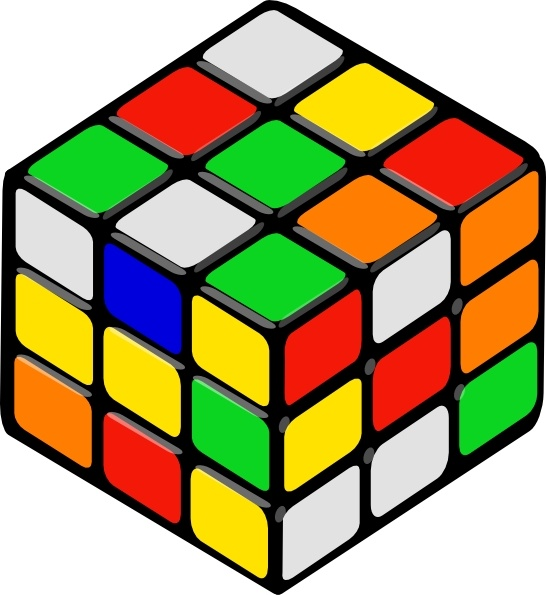
\includegraphics[scale=0.2]{images/illustrate/illus1.jpg}
    \caption{Random Image}
    \end{figure}
    
    \end{section}